% This file was created by tikzplotlib v0.9.2.
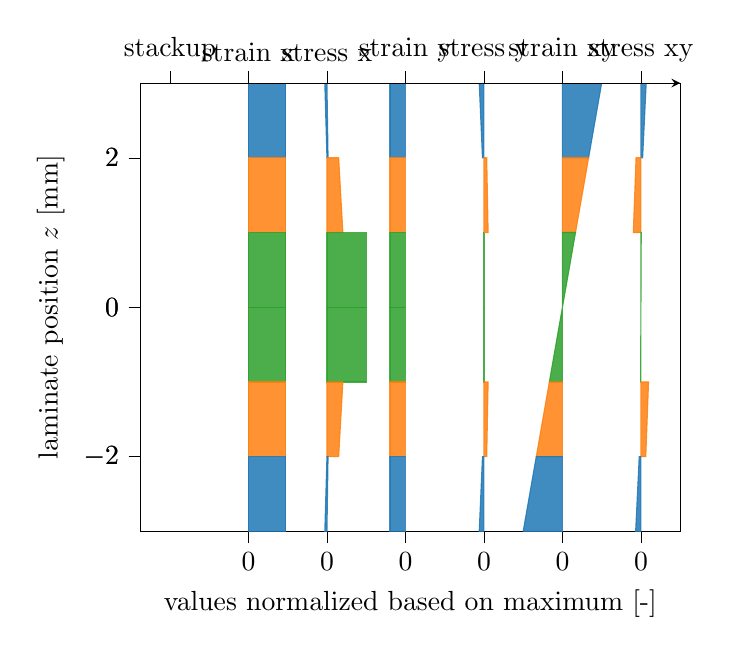
\begin{tikzpicture}

\definecolor{color0}{rgb}{0.12156862745098,0.466666666666667,0.705882352941177}
\definecolor{color1}{rgb}{1,0.498039215686275,0.0549019607843137}
\definecolor{color2}{rgb}{0.172549019607843,0.627450980392157,0.172549019607843}

\begin{axis}[
tick align=outside,
tick pos=left,
x grid style={white!69.0196078431373!black},
xlabel={values normalized based on maximum [-]},
xmin=-0.75, xmax=13,
xtick style={color=black},
xtick={2,4,6,8,10,12},
xticklabels={0,0,0,0,0,0},
y grid style={white!69.0196078431373!black},
ylabel={laminate position \(\displaystyle z\) [mm]},
ymin=-3, ymax=3,
ytick style={color=black}
]
\path [draw=color0, fill=color0, opacity=0.85]
(axis cs:2,3)
--(axis cs:2.9499671992242,3)
--(axis cs:2.9499671992242,2)
--(axis cs:2,2)
--cycle;
\path [draw=color0, fill=color0, opacity=0.85]
(axis cs:3.94530015736292,3)
--(axis cs:4,3)
--(axis cs:4.0281692780375,2)
--(axis cs:4,2)
--cycle;
\path [draw=color0, fill=color0, opacity=0.85]
(axis cs:5.60701528116418,3)
--(axis cs:6,3)
--(axis cs:6,2)
--(axis cs:5.60701528116418,2)
--cycle;
\path [draw=color0, fill=color0, opacity=0.85]
(axis cs:7.87976360478201,3)
--(axis cs:8,3)
--(axis cs:8,2)
--(axis cs:7.96263272545659,2)
--cycle;
\path [draw=color0, fill=color0, opacity=0.85]
(axis cs:10,3)
--(axis cs:11,3)
--(axis cs:10.6666666666667,2)
--(axis cs:10,2)
--cycle;
\path [draw=color0, fill=color0, opacity=0.85]
(axis cs:12,3)
--(axis cs:12.1344535103871,3)
--(axis cs:12.0434790252105,2)
--(axis cs:12,2)
--cycle;
\path [draw=color1, fill=color1, opacity=0.85]
(axis cs:2,2)
--(axis cs:2.9499671992242,2)
--(axis cs:2.9499671992242,1)
--(axis cs:2,1)
--cycle;
\path [draw=color1, fill=color1, opacity=0.85]
(axis cs:4,2)
--(axis cs:4.29823904351136,2)
--(axis cs:4.40587705137773,1)
--(axis cs:4,1)
--cycle;
\path [draw=color1, fill=color1, opacity=0.85]
(axis cs:5.60701528116418,2)
--(axis cs:6,2)
--(axis cs:6,1)
--(axis cs:5.60701528116418,1)
--cycle;
\path [draw=color1, fill=color1, opacity=0.85]
(axis cs:8,2)
--(axis cs:8.0708401215808,2)
--(axis cs:8.10673564110136,1)
--(axis cs:8,1)
--cycle;
\path [draw=color1, fill=color1, opacity=0.85]
(axis cs:10,2)
--(axis cs:10.6666666666667,2)
--(axis cs:10.3333333333333,1)
--(axis cs:10,1)
--cycle;
\path [draw=color1, fill=color1, opacity=0.85]
(axis cs:11.8760898667446,2)
--(axis cs:12,2)
--(axis cs:12,1)
--(axis cs:11.8058256540473,1)
--cycle;
\path [draw=color2, fill=color2, opacity=0.85]
(axis cs:2,1)
--(axis cs:2.9499671992242,1)
--(axis cs:2.9499671992242,0)
--(axis cs:2,0)
--cycle;
\path [draw=color2, fill=color2, opacity=0.85]
(axis cs:4,1)
--(axis cs:5,1)
--(axis cs:5,0)
--(axis cs:4,0)
--cycle;
\path [draw=color2, fill=color2, opacity=0.85]
(axis cs:5.60701528116418,1)
--(axis cs:6,1)
--(axis cs:6,0)
--(axis cs:5.60701528116418,0)
--cycle;
\path [draw=color2, fill=color2, opacity=0.85]
(axis cs:7.99001395353962,1)
--(axis cs:8,1)
--(axis cs:8,0)
--(axis cs:7.99001395353962,0)
--cycle;
\path [draw=color2, fill=color2, opacity=0.85]
(axis cs:10,1)
--(axis cs:10.3333333333333,1)
--(axis cs:10,0)
--(axis cs:10,0)
--cycle;
\path [draw=color2, fill=color2, opacity=0.85]
(axis cs:12,1)
--(axis cs:12.0081333952591,1)
--(axis cs:12,0)
--(axis cs:12,0)
--cycle;
\path [draw=color2, fill=color2, opacity=0.85]
(axis cs:2.9499671992242,0)
--(axis cs:2,0)
--(axis cs:2,-1)
--(axis cs:2.9499671992242,-1)
--cycle;
\path [draw=color2, fill=color2, opacity=0.85]
(axis cs:4,0)
--(axis cs:5,0)
--(axis cs:5,-1)
--(axis cs:4,-1)
--cycle;
\path [draw=color2, fill=color2, opacity=0.85]
(axis cs:6,0)
--(axis cs:5.60701528116418,0)
--(axis cs:5.60701528116418,-1)
--(axis cs:6,-1)
--cycle;
\path [draw=color2, fill=color2, opacity=0.85]
(axis cs:7.99001395353962,0)
--(axis cs:8,0)
--(axis cs:8,-1)
--(axis cs:7.99001395353962,-1)
--cycle;
\path [draw=color2, fill=color2, opacity=0.85]
(axis cs:10,0)
--(axis cs:10,0)
--(axis cs:9.66666666666667,-1)
--(axis cs:10,-1)
--cycle;
\path [draw=color2, fill=color2, opacity=0.85]
(axis cs:12,0)
--(axis cs:12,0)
--(axis cs:12,-1)
--(axis cs:11.9918666047409,-1)
--cycle;
\path [draw=color1, fill=color1, opacity=0.85]
(axis cs:2.9499671992242,-1)
--(axis cs:2,-1)
--(axis cs:2,-2)
--(axis cs:2.9499671992242,-2)
--cycle;
\path [draw=color1, fill=color1, opacity=0.85]
(axis cs:4,-1)
--(axis cs:4.40587705137773,-1)
--(axis cs:4.29823904351136,-2)
--(axis cs:4,-2)
--cycle;
\path [draw=color1, fill=color1, opacity=0.85]
(axis cs:6,-1)
--(axis cs:5.60701528116418,-1)
--(axis cs:5.60701528116418,-2)
--(axis cs:6,-2)
--cycle;
\path [draw=color1, fill=color1, opacity=0.85]
(axis cs:8,-1)
--(axis cs:8.10673564110136,-1)
--(axis cs:8.0708401215808,-2)
--(axis cs:8,-2)
--cycle;
\path [draw=color1, fill=color1, opacity=0.85]
(axis cs:10,-1)
--(axis cs:9.66666666666667,-1)
--(axis cs:9.33333333333333,-2)
--(axis cs:10,-2)
--cycle;
\path [draw=color1, fill=color1, opacity=0.85]
(axis cs:12,-1)
--(axis cs:12.1941743459527,-1)
--(axis cs:12.1239101332554,-2)
--(axis cs:12,-2)
--cycle;
\path [draw=color0, fill=color0, opacity=0.85]
(axis cs:2.9499671992242,-2)
--(axis cs:2,-2)
--(axis cs:2,-3)
--(axis cs:2.9499671992242,-3)
--cycle;
\path [draw=color0, fill=color0, opacity=0.85]
(axis cs:4,-2)
--(axis cs:4.0281692780375,-2)
--(axis cs:4,-3)
--(axis cs:3.94530015736292,-3)
--cycle;
\path [draw=color0, fill=color0, opacity=0.85]
(axis cs:6,-2)
--(axis cs:5.60701528116418,-2)
--(axis cs:5.60701528116418,-3)
--(axis cs:6,-3)
--cycle;
\path [draw=color0, fill=color0, opacity=0.85]
(axis cs:7.96263272545659,-2)
--(axis cs:8,-2)
--(axis cs:8,-3)
--(axis cs:7.87976360478201,-3)
--cycle;
\path [draw=color0, fill=color0, opacity=0.85]
(axis cs:10,-2)
--(axis cs:9.33333333333333,-2)
--(axis cs:9,-3)
--(axis cs:10,-3)
--cycle;
\path [draw=color0, fill=color0, opacity=0.85]
(axis cs:11.9565209747895,-2)
--(axis cs:12,-2)
--(axis cs:12,-3)
--(axis cs:11.8655464896129,-3)
--cycle;
\end{axis}

\begin{axis}[
axis x line=top,
legend cell align={left},
legend style={fill opacity=0.8, draw opacity=1, text opacity=1, at={(1.05,0.5)}, anchor=west, draw=none},
tick align=outside,
x grid style={white!69.0196078431373!black},
xmin=-0.75, xmax=13,
xtick pos=right,
xtick style={color=black},
xtick={0,2,4,6,8,10,12},
xticklabels={stackup,strain x,stress x,strain y,stress y,strain xy,stress xy},
y grid style={white!69.0196078431373!black},
ymin=-3, ymax=3,
ytick pos=left,
ytick style={color=black}
]
\end{axis}

\end{tikzpicture}
